\documentclass[12pt, a4paper, twoside]{book}
\usepackage[utf8]{inputenc}

\usepackage[top=4cm,bottom=3cm,left=4cm,right=3cm]{geometry}

\usepackage{graphicx}
\usepackage{booktabs}
\usepackage{array}
\usepackage{paralist}
\usepackage{amsmath,amssymb}
\usepackage{setspace}
\usepackage{enumitem}
\usepackage{float}
\usepackage{tikz,pgfplots}
\usepackage{multicol,multirow}
\usepackage{asymptote}
\usepackage{hyperref}
\usepackage{titlesec}
\usepackage{gensymb}
\usepackage{nicefrac}
\usepackage{fancyhdr}
\usepackage{lastpage}

\usetikzlibrary{patterns}

\newcommand{\dx}{\text{ d}x}
\newcommand{\dy}{\text{ d}y}
\newcommand{\ddv}{\text{ d}v}
\newcommand{\du}{\text{ d}u}

\renewcommand{\chaptername}{Bagian}

\fancypagestyle{plain}{
	\fancyhf{}
	\fancyhead[LE,RO]{\sffamily \thepage\ / \pageref{LastPage}}
	\renewcommand{\headrulewidth}{2pt}
}

\pagestyle{fancy}
\fancyhf{}
\fancyhead[LO]{\slshape \sffamily\rightmark}
\fancyhead[RE]{\slshape \sffamily\leftmark}
\fancyhead[LE,RO]{\sffamily \thepage\ / \pageref{LastPage}}
\renewcommand{\headrulewidth}{2pt}

\titleformat{\chapter}[display]
    {\normalfont\huge\bfseries}{\chaptertitlename\ \thechapter}{10pt}{\Huge}
\titlespacing*{\chapter}{0pt}{0pt}{40pt}

\renewcommand{\contentsname}{\hfill Daftar Isi\hfill}

\onehalfspacing
\begin{document}
\frontmatter

\clearpage
{
	\pagestyle{empty}
	\fancypagestyle{plain}
	{
		\fancyhf{}
		\fancyfoot[C]{\sffamily\thepage}
		\renewcommand{\headrulewidth}{2pt}
	}
	\tableofcontents
	\clearpage
	\begingroup
		\pagestyle{empty}%
		\begin{center}{\sffamily\bf\footnotesize \emph{HALAMAN INI SENGAJA DIKOSONGKAN}}\end{center}
		\cleardoublepage
	\endgroup
}
%%%%%%%%%%%%%%%%%%%%%%%%%%%%%%%
\mainmatter

\chapter{Kumpulan Soal Mandiri}
\hrulefill

\section{Soal Mandiri - Astramatika XXIV}
\begin{enumerate}

\item Nilai $x$ yang menyebabkan pernyataan:
	\begin{center}
	\emph{``Jika $x^2+2x = 24$ maka $x^2+4x>17$''}
	\end{center}
bernilai salah adalah \ldots

\item Jika $p$ dan $q$ adalah akar-akar persamaan $x^2-3x+4 = 0$ maka nilai $$(p^2-p+4)(q^2+q+4)$$ adalah \ldots

\item Jika $\{x\in\mathbb{R} \mid x<p \textrm{ atau } x>q\}$ merupakan himpunan penyelesaian dan memenuhi $1<a<2$ dari pertidaksamaan $${\displaystyle \frac{ax^2-3x+5}{3+8x-3x^2}\leq 0},$$maka nilai $3p+2q$ adalah \ldots

\item Absis titik balik grafik fungsi $f(x) = ax^2 + (a+6)x + 8$ adalah $-a$ dengan $a$ bilangan bulat. Nilai maksimum fungsi tersebut adalah \ldots

\item Garis $y=2x+k$ memotong parabola $y=x^2-x+3$ di titik $(a,b)$ dan $(c,d)$. Jika $a^2+c^2 = 7$ maka nilai $k$ adalah \ldots

\item Jika $${\displaystyle \sqrt{\frac{b}{a}\sqrt{\frac{a}{b}\sqrt{\frac{b}{a}\sqrt{\frac{a}{b}\cdots}}}}} = a^xb^{-x},$$ maka nilai $x$ adalah \ldots

\item Jika $a^{2x} + a^{-2x} = 3$, maka nilai dari $a^x - a^{-x}$ adalah \ldots

\item Diketahui $\log_2 56 = 7a, \log_7 2 = b, \log_4 1024 = c$ dan $${\displaystyle \left(\frac{1}{b} + \frac{50}{c}\right)^2 = d},$$ untuk $d=0$. Maka nilai $a$ adalah \ldots

\item Selisih dua bilangan positif adalah 5. Jumlah kuadratnya 2.100 kurangnya dari kuadrat jumlahnya. Jumlah kedua bilangan tersebut adalah \ldots

\item Jika $x$ adalah bilangan bulat negatif dan $3b+3x = 2a, 2x+a = b, 4a-5b = c$ dimana $a,b,$ dan $c$ adalah bilangan real. Nilai minimum dari $a+b+c$ adalah \ldots

\item Jika titik $(3,2), (11,0),$ dan $(1,k)$ terletak pada satu garis lurus, maka nilai $k$ adalah \ldots

\item Pada daerah $3x+2y \geq 24, 2x+2y\geq 20, x,y\geq 0$. Fungsi objektif $$f(x,y) = ax+4y$$ dimana $a$ adalah bilangan bulat, mencapai nilai minimum di titik $(4,6)$ jika nilai $a = \ldots$

\item Daerah definisi fungsi $$f(x) = \sqrt{\frac{x^2-x+2}{x-2}}$$ adalah \ldots

\item Diketahui $f^{-1}(8x-10) = 6x-2$ dan $(f^{-1} \circ f)(10) = p^2+4p-20$ maka hasil kali akar-akar dari $(f^{-1} \circ f)(10) = p^2+4p-20$ adalah \ldots

\item Hasil dari $\sin(\ang{2550}) + \tan(\ang{2025})$ adalah \ldots

\item Jika $${\displaystyle \sin\left(\frac{1}{2}\theta\right) = \frac{1}{5}\sqrt{5}},$$ maka $\sin(2\theta)$ adalah \ldots

\item Hasil dari $${\displaystyle \cos\left(\frac{\pi}{8}\right) + \cos\left(\frac{3\pi}{8}\right) + \cos\left(\frac{5\pi}{8}\right) + \cos\left(\frac{7\pi}{8}\right)}$$ adalah \ldots

\item Hasil dari $${\displaystyle \lim_{x\to1}\frac{(2x-3\sqrt{x}+1)(\sqrt{x}-1)}{(x-1)^2}}$$ adalah \ldots

\item Turunan pertama fungsi $f(x) = (\sin x + \cos x)^4$ adalah $f'(x)$. Nilai $f'(x)$ adalah \ldots

\item Turunan pertama $$y = -\cos(-\cos(-\cos\cdots(-\cos x)\cdots))$$ pada $x = \frac{\pi}{2}$ adalah \ldots

\item Nilai dari $$\int \sin^4(3x)\cos(3x) \dx$$ adalah \ldots

\item Daerah $D$ terletak antara garis $y=2x$, garis $x=3$, dan garis $y=0$. Volume benda putar yang terjadi jika $D$ diputar mengelilingi garis $x=3$ adalah \ldots

\item Besar sudut antara vektor $3\hat{i} + 4\hat{j} + 2\hat{k}$ dengan vektor $2\hat{i} - 3\hat{j} + 3\hat{k}$ adalah \ldots

\item Sisa pembagian $ax^{2016} - bx^{2017} - 2x+1$ oleh $x^2-1$ adalah $x+2$. Nilai $a+b$ adalah \ldots

\item Diketahui $4x^2-6px-4q$ dan $2x^2+2q$ mempunyai faktor yang sama yaitu $(x-a)$, dengan $p,q,$ dan $a$ merupakan konstanta bukan nol. Nilai dari $9p^2 + 16q$ adalah \ldots

\item Bidang $U$ dan $V$ berpotongan pada garis $g$ dengan sudut $\theta$ di titik $P$ pada bidang $U$, jarak titik $P$ dengan bidang $V$ adalah 1. Jika $\tan \theta = \nicefrac{3}{4}$, maka jarak titik $P$ dengan garis $g$ adalah \ldots

\item Rata-rata berat badan sekelompok siswa dihitung 2 kali. Pada perhitungan pertama diperoleh rata-rata 42 dan pada perhitungan kedua diperoleh rata-rata 41. Perbedaan perhitungan disebabkan kesalahan membaca data yaitu 55 dibaca 65. Banyaknya siswa pada kelompok tersebut adalah \ldots

\item Sebuah kotak berisi 5 bola kuning dan 7 bola biru. Jika diambil 3 bola sekaligus, peluang terambilnya semua bola berwarna sama adalah \ldots

\item Kedua garis lurus yang ditarik dari titik $(-1,-2)$ dan menyinggung lingkaran dengan persamaan $x^2+y^2-2x-10y+21=0$ mempunyai gradien \ldots

\item $A'(3,4)$ dan $B'(1,6)$ adalah bayangan dari $A(2,3)$ dan $B(-4,1)$ oleh transformasi $T_1 = \begin{bmatrix} a & b\\ 0 & 1\end{bmatrix}$ diteruskan $T_2 = \begin{bmatrix} 0 & 1 \\ -1 & 1\end{bmatrix}$. Nilai $3a + b$ adalah \ldots

\item Untuk 5 bilangan positif yang berbeda, jumlah setiap 4 bilangan adalah 221, 216, 214, 222, dan 211. Tentukanlah hasil dari penjumlahan bilangan terbesar dengan yang terkecil!

\item Suku ke-$n$ suatu barisan adalah $$U_n = \frac{1}{n^2+n}.$$ Tentukan nilai dari $U_1 + U_2 + U_3 +\ldots + U_{2017}$.

\item Titik $B$ dan $C$ terletak pada kurva $y=x^2$ dan $BC$ sejajar dengan sumbu-$x$. Hitunglah luas maksimum segitiga $ABC$. \par \emph{Gambarnya tidak jelas.}

\item Tentukan volume benda putar yang terbentuk dari daerah yang dibatasi oleh kurva $y=-x^2\sqrt{3},$ sumbu-$x$, didalam lingkaran $x^2+y^2=4$ diputar mengelilingi sumbu $x$.

\item Nilai semua tes matematika dinyatakan dengan bilangan bulat dari 0 sampai 10. Tentukanlah median terbesar yang mungkin bagi siswa yang memiliki rata-rata 6,5 dari enam kali tes!

\end{enumerate}

\chapter{Kumpulan Soal Kelompok}
\hrulefill

\section{Soal Kelompok - Astramatika XXIV}
\begin{enumerate}
\item Diketahui $p$ merupakan bilangan bulat positif. Jika salah satu akar persamaan $$x^2-8x+5p=0$$ empat lebih besar dari salah satu akar $$x^2-8x-3p=0,$$maka nilai $p$ adalah?

\item Tentukan himpunan penyelesaian $$\abs{\frac{3x-2}{2x+1}}\geq 3$$

\item Tentukan himpunan penyelesaian dari pertidaksamaan $$\frac{1}{\sqrt{2x+1}-\sqrt{2x}} \leq \sqrt{4x+5}$$

\item Sebuah benda ditembakkan tegak lurus ke atas. Ketinggian yang dicapai setelah $t$ detik adalah $(24t-t^2)$ meter. Tentukan berapa lama benda tersebut berada pada ketinggian tidak kurang dari 143 meter!

\item Tentukan nilai $x$ yang memenuhi $$\left(\sqrt{5-3\sqrt{3}}\right)^x - \left(\sqrt{5-3\sqrt{3}}\right)^{-x} = -\frac{8}{3}$$

\item Jika $y_1$ dan $y_2$ memenuhi persamaan $$\frac{\log_9 \frac{y^{10}}{9}}{\log_3 y} - \frac{1}{\log_y 3} = \frac{5}{\log_3 y}.$$ Tentukan nilai dari $\frac{2}{3}(y_1+y_2)$.

\item Bila diketahui $a+b=3ab$,\ $b+c=9bc$, dan $a+c=7ac$. Tentukan nilai dari $a+b+c$.

\item Anggota pramuka akan mengadakan perkemahan disuatu kawasan dan mereka mengumpulkan uang sama banyaknya untuk membayar harga sewa mini bus sebesar Rp2.115.000,00, tiket masuk sebesar Rp40.000,00, dan biaya administrasi sebesar Rp5.000,00. Karena ada empat orang yang batal berangkat, maka setiap anggota yang berangkat harus menambah Rp18.000,00. Tentukan banyaknya anggota yang berangkat!

\item Tentukan nilai $a+c$, jika himpunan penyelesaian dari $$x-y=1\text{ dan }x^2+4xy-2y^2 = 18$$ adalah $\{(a,b), (c,d)\}$.

\item Seorang penjahit mempunyai persediaan 2 meter kain merah, 3 meter kain biru dan 4 meter kain hitam. Penjahit tersebut membuat 2 jenis pakaian untuk dijual. Pakaian model A memerlukan 20 cm kain merah, 50 cm kain biru dan 80 cm kain hitam.  Sedangkan model B memerlukan 50 cm kain merah, 60 cm kain biru dan 50 cm kain hitam. Pakaian model A dijual Rp120.000,00 dan pakaian model B dijual seharga Rp100.000,00. Tentukan banyaknya pakaian A dan B yang dijual untuk mencapai penjualan maksimum!

\item Tentukan nilai minimum dari fungsi $$f(x) = \frac{1}{\sqrt{3}\sin(3x) - \sqrt{13}\cos(3x)+8}.$$

\item $x_1$ dan $x_2$ adalah bilangan bulat yang merupakan akar-akar dari persamaan $$2x^2 - (3k^2-2k+2)x + 6k-4 = 0$$ dimana $x_1<x_2$. Jika $x_1,\ k,\ x_2$ merupakan tiga suku pertama suatu barisan geometri. Tentukan selisih dari jumlah 10 suku pertama dengan jumlah 6 suku pertama!

\item Suatu barisan geometri semua sukunya positif. Jika $$\frac{u_3+u_4}{u_1+u_2} = \frac{1}{16},$$ tentukan nilai dari $$\frac{u_1+u_2+u_3+u_4}{u_2+u_3}$$

\item Tentukan nilai dari $$\lim_{x\to\infty}(3^x + 3^{3x})^{\frac{1}{x}}$$

\item Diketahui $f(x) = \tan^2(3x-2)$. Tentukan nilai $$\lim_{h\to\infty}h\left[\left(f^\prime\left(x+\frac{1}{h}\right)-f^\prime(x)\right)\right]$$

\item Tentukanlah jarak terpendek titik $(4,2)$ dengan parabola $y^2=8x$.

\item Tentukanlah luas daerah yang dibatasi oleh parabola $y=x^2-9$ dan garis $y=-4\abs{x}$.

\item Tentukan $$\int \sqrt{1-\tan^2(4x)+\tan^{4}(4x)-\tan^6(4x)+\ldots}\dx$$

\item Untuk vektor $\vec{a}\cdot\vec{b}$ dan $\vec{c} = 3\vec{a}+2\vec{b}$. Jika $\abs{\vec{a}} = 2$, $\abs{\vec{b}} = 3$, dan sudut $\left(\vec{a},\vec{b}\right) = \ang{120}.$ Tentukan nilai $\abs{\vec{c}}$.

\item Tentukan nilai hasil kali akar-akar pertidaksamaan $$(1-5x)(1-8x)(1-2x)(1+30x) - 2$$

\item Di dalam suatu drum berbentuk tabung dengan diameter 36 cm dan tinggi 70 cm dimasukkan bola besi berjari-jari 12 cm, kemudian dimasukkan lagi bola besi berjari-jari 8 cm. Drum tersebut diisi air sehingga kedua bola terendam. Minimal volume air yang diperlukan?

\item Suatu kerucut tegak tertutup berisi air memiliki diameter alas 6 cm dan tinggi $t$ cm. Tinggi air dalam kerucut adalah $\frac{1}{4}t$ cm. Jika posisi tersebut dibalik, berapakah ketinggian air dalam kerucut?

\item Dalam perhitungan rata-rata hasil ulangan 36 siswa, nilai seorang siswa dimasukkan hanya $\frac{3}{4}$ dari nilai sebenarnya sehingga rata-rata yang diperoleh selisih 0,5 poin dari rata-rata sebenarnya. Tentukan nilai seorang siswa tersebut!

\item Vera akan menyusun enam buku matematika, dua buku ekonomi, dan 2 buku bahasa. Buku-buku tersebut akan disusun di lemari buku dalam satu baris. Misalkan $A$ adalah kejadian \emph{``tidak ada 2 atau lebih buku sejenis tersusun berurutan''}, tentukanlah peluang kejadian $A$.

\item Dari huruf alfabet dipilih satu per satu 11 huruf sembarang dengan cara pengambilan secara acak dan disusun sehingga membentuk suatu kata. Tentukan peluang kata yang terbentuk adalah \emph{ASTRAMATIKA} dalam satu rangkaian!

\item Garis $3x+4y = 7$ memotong lingkaran $x^2+y^2-6x-2y+2=0$ di titik $P$ dan $Q$. Tentukan panjang ruas garis $PQ$.

\item Dua lingkaran identik berjari-jari 5 cm saling berpotongan. Jika lingkaran pertama melalui titik pusat lingkaran yang kedua, tentukanlah luas daerah irisannya!

\item $ABCD$ merupakan bangun layang-layang dengan diketahui koordinat titik $A(-2,-1)$, $B(1,-1)$, dan $C(3,4)$. Jika diketahui koordinat $D$ oleh refleksi terhadap sumbu $y$ adalah $D'(2,2)$. Tentukan luas layang-layang $ABCD$ jika didilatasikan terhadap $(0,2)$!

\item Diketahui determinan dari hasil perkalian matriks $$P=\begin{bmatrix}0&2\\3&1\end{bmatrix}$$ dengan matriks $$Q=\begin{bmatrix}2&1\\3&1\end{bmatrix}$$ merupakan diameter lingkaran $g$ yang berpusat di titik $(0,0)$. Jika garis $h$ yang merupakan garis singgung lingkaran $l$ dan melalui titik potong antara garis $y+7x-10=0$ dengan garis $y=10x+10$, tentukan persamaan garis $l$.

\item Jika $$A=\begin{bmatrix}\nicefrac{2}{3} & \nicefrac{2}{3} & a\\ \nicefrac{1}{3} & b & \nicefrac{2}{3}\\ c & -\nicefrac{1}{3} & -\nicefrac{2}{3}\end{bmatrix}$$ adalah matrix orthogonal. Tentukan nilai dari $a^2+b^2+c^2$.
\end{enumerate}
\clearpage
	\begingroup
		\pagestyle{empty}%
		\begin{center}{\sffamily\bf\footnotesize \emph{HALAMAN INI SENGAJA DIKOSONGKAN}}\end{center}
		\cleardoublepage
	\endgroup
\chapter{Pembahasan Soal Mandiri}
\hrulefill

\section{Soal Mandiri - Astramatika XXIV}
\begin{enumerate}

\item \textbf{Jawaban: -6.} Kita lihat dari kata \emph{``Jika $x^2+2x=24$ \ldots''}, didapat $$x^2+2x-24 = 0\Leftrightarrow (x+6)(x-4) = 0$$nilai $x$ yang memenuhi adalah $x=-6$ dan $x=4$. Kemudian kita substitusikan ke pertidaksamaan pada kata \emph{``\ldots maka $x^2+4x>17$''}, saat $x = -6$ didapat $$x^2 + 4x = (-6)^2 + 4(-6) = 36 - 24 = 12 < 17$$kemudian saat $x=4$ didapat $$x^2+4x = (4)^2 + 4(4) = 32 > 17$$maka nilai $x$ yang membuat pernyataan pada soal bernilai salah adalah $x=-6$.

\item \textbf{Jawaban: 32.} Karena $p,q$ adalah akar-akar persamaan $x^2-3x+4=0,$ maka $$p^2-3p+4 =0\Leftrightarrow p^2-p+4 = 2p$$kemudian$$q^2-3q+4 = 0\Leftrightarrow q^2+q+4=4q$$lalu dari formula vieta, kita tahu bahwa $pq = 4$, sehingga didapat $$(p^2-p+4)(q^2-3q+4) = (2p)(4q) = 8pq = 32$$

\item \textbf{Jawaban: 5.} Perhatikan bentuk $ax^2-3x+5$, bentuk persamaan kuadrat tersebut memiliki nilai diskriminan $$D = b^2-4ac = 9-20a < 0\text{ untuk $1<a<2$}$$yang membuat bentuk kuadrat $ax^2-3x+5$ definit positif. Maka agar pertidaksamaan pada soal dapat terpenuhi, haruslah \begin{equation}-3x^2+8x+3 = (3x+1)(3-x) < 0\end{equation}bisa dicek bahwa solusi dari (III.1) adalah $x<-\nicefrac{1}{3}$ dan $x>3$. Maka $(p,q) = (-\nicefrac{1}{3}, 3)$, sehingga nilai dari $3p +2q = 3(-\frac{1}{3}) + 2(3) = 5.$

\item \textbf{Jawaban: 8.} Titik balik fungsi kuadrat adalah titik $x$ yang memenuhi $f'(x) = 0$ dengan $f'(x)$ menyatakan turunan pertama fungsi $f(x)$. Oleh karena itu, berarti $x=-a$ memenuhi $f'(-a) = 0$, sehingga dengan $$f'(x) = 2ax + (a+6)$$didapat$$f'(-a) = 2a(-a)+(a+6) = -2a^2+a+6 = (2a+3)(2-a) = 0$$karena $a$ bilangan bulat, maka $a=2$. Berarti $$f(x) = 2x^2+8x+8 = 2(x+2)^2$$kemudian karena $0\leq (x+2)^2 \leq 4$, maka $$0\leq f(x)\leq 8$$ yang berarti nilai maksimum $f(x)$ adalah 8, yang terjadi saat $x=0$.

\item \textbf{Jawaban: 2.} Karena garis $y=2x+k$ dan parabola $y=x^2-x+3$ saling berpotongan, maka \setcounter{equation}{0}\begin{equation}2x+k = x^2-x+3 \Leftrightarrow x^2-3x+(3-k) = 0.\end{equation} \par Dari soal kita tahu bahwa $a^2 + c^2 = 7$, yang berarti $$a^2 + c^2 = (a+c)^2 - 2ac = 7.$$\par Sekarang, karena $a,c$ memenuhi (III.1), maka $a+c = 3$ dan $ac = 3-k$, sehingga didapat $$(a+c)^2-2ac = 9-6+2k = 3+2k = 7\Leftrightarrow k = 2.$$

\item \textbf{Jawaban: $-\nicefrac{1}{3}.$} Perhatikan bahwa $$\sqrt{\frac{b}{a}\sqrt{\frac{a}{b}\sqrt{\frac{b}{a}\sqrt{\frac{a}{b}\cdots}}}} = \sqrt{\frac{b}{a}\sqrt{\frac{a}{b}\cdot \frac{a^x}{b^x}}} = \sqrt{\frac{b}{a}\sqrt{\frac{a^{x+1}}{b^{x+1}}}} = \frac{a^x}{b^x}$$kemudian$$\sqrt{\frac{a^{x+1}}{b^{x+1}}} = \frac{a^{2x+1}}{b^{2x+1}}\Leftrightarrow \frac{a^{x+1}}{b^{x+1}} = \frac{a^{4x+2}}{b^{4x+2}}$$kemudian didapat $$\frac{a^{3x+1}}{b^{3x+1}} = 1$$yang hanya dapat terjadi jika $3x+1 = 0$ karena $a\neq b$, maka $x=-\nicefrac{1}{3}$.

\item \textbf{Jawaban: $\pm$1.} Perhatikan bahwa $$(a^x - a^{-x})^2 = (a^{2x} + a^{-2x}) - 2 = 3-2 = 1$$maka didapat $a^x - a^{-x} = \pm1.$

\item \textbf{Jawaban: -1.} Perhatikan bahwa $$\log_2 56 = \log_2 (2^3)(7) = 3+\log_2 7 = 7a$$kemudian karena $\log_7 2 = b\Leftrightarrow \log_2 7 = \nicefrac{1}{b}$, maka didapat \setcounter{equation}{0}\begin{equation}3+\frac{1}{b} = 7a.\end{equation}Kemudian karena $c = \log_4 1024 = 5$, maka $$\left(\frac{1}{b} + \frac{50}{c}\right)^2 = \left(\frac{1}{b} + 10\right)^2 = d = 0$$yang berarti $\nicefrac{1}{b} = -10.$ Substitusikan $\nicefrac{1}{b} = -10$ ke (III.1) didapat $$3 - 10 = -7 = 7a\Leftrightarrow a = -1.$$

\item \textbf{Jawaban: 65.} Misalkan dua bilangan tersebut adalah $x,y$ dengan $x>y$. Maka
	\setcounter{equation}{0}\begin{gather}
	x-y = 5\\
	x^2+y^2 = (x+y)^2 - 2100
	\end{gather}
dari (III.2) didapat $xy = 1050$, kemudian $$x^2+y^2 = (x-y)^2+2xy = (5)^2 + 2(1050) = 2125$$sehingga didapat $$(x+y)^2 = (x^2+y^2) + 2xy = (2125)+2(1050) = 4225\Leftrightarrow  x+y = 65$$

\item \textbf{Jawaban: 17.} Dari soal diketahui
	\setcounter{equation}{0}\begin{gather}
	3b+3x = 2a\\
	2x+a = b\\
	4a-5b = c
	\end{gather}
substitusi (III.2) ke (III.1), didapat $$ 3(2x+a) + 3x= 9x + 3a = 2a\Leftrightarrow a = -9x \geq 9\text{ karena $x\leq -1.$}$$Selanjutnya, dari (III.2) didapat $a = b-2x$, subsitusikan ke (III.1) didapat $$3b+3x = 2(b-2x) = 2b-4x\Leftrightarrow b = -7x \geq 7\text{ karena $x\leq-1.$}$$Terakhir, subsitusikan $a=-9x$ dan $b=-7x$ ke (III.3) sehingga didapat $$4a-5b = 4(-9x) - 5(-7x) = 35x - 36x = -x = c\geq 1\text{ karena $x\leq -1$,}$$sehingga nilai minimum dari $a+b+c$ adalah $$a+b+c \geq 9 + 7 + 1 = 17.$$

\item \textbf{Jawaban: $\nicefrac{5}{2}$.} Tiga titik $(x_1,y_1),(x_2,y_2),$ dan $(x_3,y_3)$ segaris jika $$\frac{x_2 - x_1}{y_2 - y_1} = \frac{x_3 - x_2}{y_3 - y_2}$$sehingga, karena titik $(3,2),(11,0),$ dan $(1,k)$ segaris, maka haruslah $$\frac{11-3}{0-2} = \frac{1-11}{k}\Leftrightarrow -4 = \frac{-10}{k}\Leftrightarrow k = \frac{5}{2}.$$

\item \textbf{Jawaban: 5.} Daerah yang diarsir pada gambar dibawah menunjukkan daerah penyelesaian dari sistem pertidaksamaan pada soal.
	\begin{figure}[H]
		\centering
		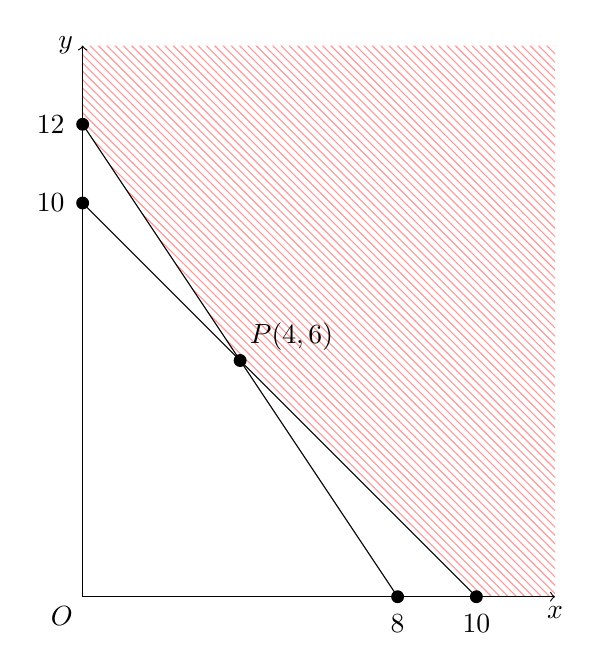
\begin{tikzpicture}[scale = 0.5]
			\fill[pattern color = red!40, pattern = north west lines] (0,14)--(12,14)--(12,0)--(10,0)--(4,6)--(0,12)--cycle;
			
			\draw[->] (0,0) -- (12,0)node[anchor = north]{$x$}; % x axis
			\draw[->] (0,0) -- (0,14)node[anchor = east]{$y$}; % y axis
			
			\node[draw, circle, fill = black, inner sep = 1.5] at (10,0){};
			\node[draw, circle, fill = black, inner sep = 1.5] at (0,10){};
			
			\node[anchor = north, yshift = -3] at (10,0){10};
			\node[anchor = east, xshift = -3] at (0,10){10};
			\node[anchor = north east] at (0,0) {$O$};
			
			\node[draw, circle, fill = black, inner sep = 1.5] at (8,0){};
			\node[draw, circle, fill = black, inner sep = 1.5] at (0,12){};
			
			\node[anchor = north, yshift = -3] at (8,0){8};
			\node[anchor = east, xshift = -3] at (0,12){12};
			
			\node[draw, circle, fill = black, inner sep = 1.5] at (4,6){};
			\node[anchor = south west] at (4,6){$P(4,6)$};
			
			\draw (10,0)--(0,10){};
			\draw (8,0)--(0,12){};
		\end{tikzpicture}
	\end{figure}
karena fungsi $f(x,y) = ax + 4y$ berada pada daerah yang diarsir, atau daerah penyelesaian sistem pertidaksamaan pada soal. Maka nilai $f(x,y)$ akan minimum pada salah satu titik $(10,0), (0,12),$ atau $(4,6)$. Perhatikan tabel dibawah
	\begin{center}
		\begin{tabular}{|c|c|}
		\hline
		$(x,y)$ & $f(x,y)$\\
		\hline
		$(10,0)$ & 10a\\
		\hline
		$(0,12)$ & 48\\
		\hline
		$(4,6)$ & 4a + 24\\
		\hline 
		\end{tabular}
	\end{center}
karena $f(x,y)$ minimum saat $(x,y) = (4,6)$, maka haruslah $$f(10,0) = 10a > f(4,6) = 4a + 24\Leftrightarrow a > 4$$ dan juga $$f(0,12) = 48 > f(4,6) = 4a + 24\Leftrightarrow a < 6$$sehingga haruslah $a=5$.

\item \textbf{Jawaban: $\{x\in\mathbb{R}\mid x>2\}$.} Syarat pertama agar fungsi $f(x)$ terdefinisi adalah $x-2 \neq 0$, sehingga $x\neq 2$. Kemudian syarat yang lain adalah, \setcounter{equation}{0}\begin{equation}\frac{x^2-x+2}{x-2} \geq 0,\end{equation}selanjutnya perhatikan bahwa diskriminan dari $x^2-x+2$ adalah $$D = b^2-4ac = 1 - 8 = -7 < 0$$yang berarti $x^2-x+2$ definit positif. Maka agar (III.1) dapat terpenuhi, haruslah $x-2 > 0$ atau $x>2$. Maka daerah definisi fungsi $f(x)$ adalah $\{x\in\mathbb{R}\mid x>2\}$.

\item \textbf{Jawaban: -30.} Dari $f^{-1}(8x-10) = 6x - 2$, kita substitusikan $x\rightarrow \frac{1}{8}x + \frac{5}{4}$ sehingga \setcounter{equation}{0}\begin{equation}f^{-1}\left(8\left(\frac{1}{8}x + \frac{5}{4}\right)-10\right) = f^{-1}(x) = 6\left(\frac{1}{8}x + \frac{5}{4}\right)-2 = \frac{3}{4}x + \frac{11}{2}.\end{equation}Kemudian dari definisi invers fungsi $f(x)$, yaitu $f^{-1}(f(x)) = x$. Kita dapat mencari fungsi $f(x)$ sebagai berikut, substitusikan $x\rightarrow f(x)$ didapat $$f^{-1}(f(x)) = x = \frac{3}{4}f(x) + \frac{11}{2}\Leftrightarrow f(x) = \frac{4x-22}{3}$$sehingga $$f(10) = \frac{4(10)-22}{3} = 6$$yang membuat $$(f^{-1}\circ f)(10) = f^{-1}(6) = \frac{3}{4}(6) + \frac{11}{2} = 10$$sehingga $$p^2-4p-20 = 10\Leftrightarrow p^2-4p-30 = 0.$$Maka berdasarkan formula vieta, hasil kali akar-akarnya adalah -30.

\item \textbf{Jawaban: $\nicefrac{3}{2}$.} Ingat bahwa $$\sin(\ang{360} + x) = \sin x\quad\text{dan}\quad\tan(\ang{180} +x) = \tan x$$kemudian karena$$\ang{2550} = \ang{360}\times7 + \ang{30}\quad\text{dan}\quad\ang{2025} = \ang{180}\times11 + \ang{45}$$maka$$\sin(\ang{2550}) + \tan(\ang{2025}) = \sin(\ang{30}) + \tan(\ang{45}) = \frac{1}{2} + 1 = \frac{3}{2}$$

\item \textbf{Jawaban: $\nicefrac{24}{25}$.} Perhatikan bahwa $$\cos\left(\frac{1}{2}\theta\right) = \sqrt{1-\left(\frac{\sqrt{5}}{5}\right)^2} = \frac{2}{5}\sqrt{5}.$$ Dengan menggunakan $$\sin(2x) = 2\sin(x)\cos(x)$$ beberapa kali, didapat $$\sin\left(2\times\frac{1}{2}\theta\right) = \sin(\theta) =2\sin\left(\frac{1}{2}\theta\right)\cos\left(\frac{1}{2}\theta\right) = 2\times\frac{1}{5}\sqrt{5}\times\frac{2}{5}\sqrt{5} = \frac{4}{5}$$kemudian, dari $\sin(\theta) = \nicefrac{4}{5}$ didapat $$\cos(\theta) = \sqrt{1-\left(\frac{4}{5}\right)^2} = \frac{3}{5}$$sehingga $$\sin(2\theta) = 2\sin(\theta)\cos(\theta) = 2\times\frac{4}{5}\times\frac{3}{5} = \frac{24}{25}.$$

\item \textbf{Jawaban: 0.} Ingat bahwa $$\cos(x) + \cos(y) = 2\cos\left(\frac{x+y}{2}\right)\cos\left(\frac{x-y}{2}\right)$$sehingga soal dapat diubah menjadi \setcounter{equation}{0}\begin{equation}\left(\cos\left(\frac{\pi}{8}\right) + \cos\left(\frac{5\pi}{8}\right)\right) + \left(\cos\left(\frac{3\pi}{8}\right)+\cos\left(\frac{7\pi}{8}\right)\right)\end{equation}kemudian (III.1) menjadi
	$$
	2\cos\left(\frac{\pi}{4}\right)\left(\cos\left(\frac{3\pi}{8}\right)+\cos\left(\frac{5\pi}{8}\right)\right)=2\cos\left(\frac{\pi}{4}\right)\left(2\cos\left(\frac{\pi}{2}\right)						\cos\left(\frac{\pi}{8}\right)\right).
	$$
Karena ada faktor $\cos\left(\frac{\pi}{2}\right)$ di sebelah kanan yang sama dengan nol, maka (III.1) sama dengan nol.

\item \textbf{Jawaban: $\nicefrac{1}{4}$.} Perhatikan bahwa
\begin{eqnarray*}
\frac{(2x-3\sqrt{x} +1)(\sqrt{x}-1)}{(x-1)^2} &=& \frac{(2\sqrt{x}-1)(\sqrt{x}-1)(\sqrt{x}-1)}{\left[(\sqrt{x}-1)(\sqrt{x}+1)\right]^2}\\
							 &=& \frac{(2\sqrt{x}-1)(\sqrt{x}-1)^2}{(\sqrt{x}-1)^2(\sqrt{x}+1)^2}\\
							 &=& \frac{2\sqrt{x}-1}{(\sqrt{x}+1)^2}
\end{eqnarray*}
sehingga $$\lim_{x\to1}\frac{(2x-3\sqrt{x} +1)(\sqrt{x}-1)}{(x-1)^2} = \lim_{x\to1}\frac{2\sqrt{x}-1}{(\sqrt{x}+1)^2} = \frac{2(1)-1}{((1)+1)^2} = \frac{1}{4}$$

\item \textbf{Jawaban: $4(\sin x+\cos x)^3(\cos x-\sin x)$.} Misalkan $$\sin x + \cos x = g(x)\longrightarrow g'(x) = \cos x - \sin x,$$maka dengan aturan rantai $$f(x) = [g(x)]^4 \longrightarrow f'(x) = 4[g(x)]^3g'(x)$$sehingga$$f'(x) = 4(\sin x +\cos x)^3(\cos x - \sin x)$$

\item \textbf{Jawaban: 0.} Misalkan $f'(x)$ menyatakan turunan pertama dari $f(x)$. Kemudian misalkan $$f_n(x) = \underbrace{(f_1\circ f_1\circ\cdots\circ f_1)}_{\text{$f_1$ muncul $n$ kali}}(x)$$dengan $f_1(x) = -\cos x$, contohnya $$f_2(x) = -\cos(-\cos(x))\quad\text{dan}\quad f_3(x) = -\cos(-\cos(-\cos(x))).$$ Dengan definisi diatas, soal dapat dinyatakan dengan $$L = \eval{\lim_{n\to\infty}f'_n(x)}_{x=\frac{\pi}{2}}.$$Perhatikan bahwa dengan aturan rantai $$f'_2(x) = \frac{\text{d}f_2(x)}{\text{d}f_1(x)}\cdot\frac{\text{d}f_1(x)}{\text{d}x}\quad\text{dan}\quad f'_3(x) = \frac{\text{d}f_3(x)}{\text{d}f_2(x)}\cdot\frac{\text{d}f_2(x)}{\text{d}f_1(x)}\cdot\frac{\text{d}f_1(x)}{\text{d}x},$$sehingga $$L = \eval{\lim_{n\to\infty}\frac{\text{d}f_n(x)}{\text{d}f_{n-1}(x)}\cdot\frac{\text{d}f_{n-1}(x)}{\text{d}f_{n-2}(x)}\cdots\frac{\text{d}f_2(x)}{\text{d}f_1(x)}\cdot\frac{\text{d}f_1(x)}{\text{d}x}}_{x=\frac{\pi}{2}}.$$Dari bentuk diatas, jika kita tinjau \setcounter{equation}{0}\begin{equation}\frac{\text{d}f_2(x)}{\text{d}f_1(x)} = \frac{\text{d}}{\text{d}(-\cos x)}(-\cos(-\cos x)) = \sin(-\cos x)\end{equation}saat $x=\frac{\pi}{2}$, persamaan (III.1) bernilai $$\sin\left(-\cos\frac{\pi}{2}\right) = 0$$sehingga didapat $$L = 0$$

\item \textbf{Jawaban: $\frac{1}{15}\sin^5(3x) + C$.} Misalkan $$\sin(3x) = u\longrightarrow 3\cos(3x)\dx = \du$$sehingga$$\int \sin^4(3x)\cos(3x)\dx = \frac{1}{3}\int u^4\du = \frac{1}{15}u^5 + C = \frac{1}{15}\sin^5(3x)+C$$untuk suatu $C\in\mathbb{R}$.

\item \textbf{Jawaban: $18\pi$.} Titik potong $y = 2x$ dan $x=3$ adalah $(x,y) = (3,6)$. Sehingga jika diputar mengelilingi garis $x=3$, volumenya adalah $$V = \pi\int_{0}^{6} \left(\frac{y}{2}\right)^2\dy = \pi\left[\frac{1}{12}y^3\right]_0^6 = \frac{216\pi}{12} =18\pi$$

\item \textbf{Jawaban: $\ang{90}$.} Misalkan $\vec{A} = 3\hat{i} + 4\hat{j} + 2\hat{k}$ dan $\vec{B} = 2\hat{i} - 3\hat{j} + 3\hat{k}$. Ingat bahwa $$\vec{A}\cdot\vec{B} = |A||B|\cos{\theta}$$dengan $\theta$ menyatakan sudut antara vektor $\vec{A}$ dan $\vec{B}$ yang berarti $$\cos\theta = \frac{\vec{A}\cdot\vec{B}}{|A||B|}.$$Perhatikan bahwa $$\vec{A} \cdot \vec{B} = 6 + (-12) + 6 = 0$$sehingga $\cos\theta = 0$ atau $\theta = \ang{90}$.

\item \textbf{Jawaban: -2.} Misalkan $$f(x) = ax^{2016} - bx^{2017} - 2x + 1,$$perhatikan bahwa $f(x)$ dapat dinyatakan sebagai berikut \setcounter{equation}{0}\begin{equation}f(x) = (x^2-1)P(x) + (x+2)\end{equation} untuk suatu polinomial $P(x)$. Kemudian perhatikan bahwa dari (III.1) didapat $$f(-1) = 1$$kemudian nilai dari $a+b$ dapat kita cari sebagai berikut $$f(-1) = a(-1)^{2016} - b(-1)^{2017} - 2(-1) +1 = a+b +3 = 1$$sehingga $a+b = -2.$

\item \textbf{Jawaban: 0.} Kita tinjau polinom $f(x) = 4x^2-6px -4q$ terlebih dahulu. Misalkan $f(x)$ dinyatakan dengan $$2(x-a)(2x-b) \equiv 4x^2-6px - 4q = f(x)$$dengan $\nicefrac{b}{2}$ merupakan akar dari $f(x)$. Perhatikan bahwa $$2(x-a)(2x-b) = 2(2x^2-x(2a+b)+ab)\equiv 2(2x^2-3px-2q)$$sehingga kita dapatkan sistem persamaan
	\setcounter{equation}{0}\begin{gather}
	2a + b = 3p\\
	ab = -2q.
	\end{gather}
Kemudian selanjutnya, kita tinjau polinom $g(x) = 2x^2+2q$. Sama seperti sebelumnya, misalkan $g(x)$ dapat dinyatakan dengan $$2(x-a)(x-c) \equiv 2x^2+2q = g(x)$$ dengan $c$ merupakan akar dari polinom $g(x)$. Perhatikan bahwa $$2(x-a)(x-c) = 2(x^2-x(a+c)+ac) \equiv 2(x^2+q)$$ sehingga kita dapat sistem persamaan
	\begin{gather}
	a+c = 0\\
	ac = q
	\end{gather}
dari (III.3) kita dapat $-a = c$, sehingga $a^2 = -q$. Subsitusikan $a^2=-q$ ke (III.2), didapat $$ab = 2a^2\Leftrightarrow b = 2a\quad\text{karena $a\neq 0$}$$selanjutnya, subsitusikan $b = 2a$ ke (III.1) sehingga didapat $$p = \frac{4}{3}a.$$Dengan menggunakan semua hasil diatas, didapat $$9p^2 + 16q = 9\left(\frac{16}{9}a^2\right) + 16(-a^2) = 0.$$

\item

\item \textbf{Jawaban: $10p, p\in\mathbb{N}$.} Misalkan $S_1$ dan $S_2$ menyatakan jumlah data berat badan siswa pada perhitungan pertama dan kedua berturut-turut. Maka $$S_1 = \underbrace{65+65+\ldots+65}_{\text{p kali}} + x$$dengan $x$ menyatakan jumlah data selain data yang salah dan $p$ menyatakan jumlah siswa yang datanya salah terbaca. Kemudian perhatikan bahwa karena $$S_2 = \underbrace{55+55+\ldots+55}_{\text{p kali}} + x$$maka didapat hubungan antara $S_1$ dan $S_2$ adalah \setcounter{equation}{0}\begin{equation}S_1 = S_2 + \underbrace{10+10+\ldots+10}_{\text{p kali}} = S_2 + 10p.\end{equation}Dengan meninjau rata-ratanya, dengan $n$ menyatakan banyak siswa $$\frac{S_1}{n} = 42\quad\text{dan}\quad\frac{S_2}{n} = 41$$perhatikan bahwa $$\frac{S_1}{n} - 1 = \frac{S_2}{n} = 41$$sehingga didapat $$\frac{S_1 - S_2}{n} = 1\Leftrightarrow S_1 - S_2 = n.$$ Dari (III.1) didapat $S_1 - S_2 = 10p$ sehingga $$n = 10p\quad\text{dengan sembarang $p\in\mathbb{N}$}$$

\item \textbf{Jawaban: $\nicefrac{9}{44}$.} Kita bagi menjadi beberapa kasus.
	\begin{enumerate}
	\item Terambil 3 bola kuning sekaligus:
		\par Banyak cara terambil 3 bola kuning sekaligus adalah $$\binom{5}{3} = 10\text{ cara,}$$sehingga peluangnya adalah $$P(A) = \frac{10}{\binom{5+7}{3}} = \frac{10}{220} = 		\frac{1}{22}$$
	\item Terambil 3 bola biru sekaligus:
		\par Banyak cara terambil 3 bola biru sekaligus adalah $$\binom{7}{3} = 35\text{ cara,}$$sehingga peluangnya adalah $$P(B) = \frac{35}{\binom{5+7}{3}} = \frac{35}{220} = 				\frac{7}{44}$$
	\end{enumerate}
Maka peluang terambil 3 bola berwarna sama sekaligus adalah $$P = P(A) + P(B) = \frac{1}{22} + \frac{7}{44} = \frac{9}{44}$$

\item \textbf{Jawaban: $-14\pm4\sqrt{15}$.} Kita akan menggunakan persamaan \setcounter{equation}{0}\begin{equation}y_1 - y_p = m(x_1-x_p) \pm r\sqrt{m^2+1}\end{equation}dimana $(x_1,y_1),(x_p,y_p), r,$ dan $m$ adalah titik (-1,-2), titik pusat lingkaran, jari-jari lingkaran dan gradien garis singgung yang melewati titik (-1,-2) berturut-turut. Dari persamaan lingkaran pada soal, didapat $$x^2+y^2 - 2x - 10y + 21 = 0\Leftrightarrow (x-1)^2 + (y-5)^2 = 5$$sehingga didapat titik pusat lingkaran (1,5) dan jari-jarinya $\sqrt{5}$. Dengan menggunakan persamaan (III.1) diatas,
	\begin{eqnarray*}
	\text{(III.1)} = -2 - 5 &=& m(-1 -1)\pm \sqrt{5}\times\sqrt{m^2+1}\\
			-7 &=& -2m \pm \sqrt{5m^2+5}\\
			(2m - 7)^2 &=& 5m^2+5\\
			4m^2-28m+49 &=& 5m^2+5\\
			\Leftrightarrow m^2+28m-44 &=& 0
	\end{eqnarray*}
bisa dicek bahwa solusi dari persamaan kuadrat diatas adalah $$(m_1, m_2) = (4\sqrt{15}-14, -4\sqrt{15}-14)$$sehingga gradien garis singgungnya adalah $$m = -14\pm4\sqrt{15}$$

\item \textbf{Jawaban: 2.} Kita tinjau titik $A(2,3)$ terlebih dahulu $$T_1 \longrightarrow \begin{pmatrix}a & b\\0 & 1\end{pmatrix}\times\begin{pmatrix}2\\3\end{pmatrix} = \begin{pmatrix}2a + 3b\\3\end{pmatrix}$$kemudian$$T_2\longrightarrow \begin{pmatrix}0 & 1\\ -1 & 1\end{pmatrix}\times\begin{pmatrix}2a + 3b\\ 3\end{pmatrix} = \begin{pmatrix}3 \\ -2a-3b+3\end{pmatrix}$$sehingga didapat $(3, 3-2a-3b) = (3,4)$ sehingga \setcounter{equation}{0}\begin{equation}2a+3b = -1.\end{equation} Kemudian kita tinjau titik $B(-4,1)$, $$T_1 \longrightarrow \begin{pmatrix} a & b\\ 0 & 1\end{pmatrix}\times\begin{pmatrix}-4\\1\end{pmatrix} = \begin{pmatrix}b - 4a\\1\end{pmatrix}$$kemudian$$T_2 \longrightarrow \begin{pmatrix} 0&1\\-1&1\end{pmatrix}\times\begin{pmatrix}b-4a\\1\end{pmatrix} = \begin{pmatrix}1 \\ 4a -b +1\end{pmatrix}$$sehingga didapat $(1,6) = (1, 4a-b+1)$ sehingga \begin{equation}4a-b = 5.\end{equation}Dengan menyelesaikan sistem persamaan (III.1) dan (III.2) didapat $$(a,b) = (1,-1)$$ sehingga nilai $$3a+b = 3 + (-1) = 2.$$

\item \textbf{Jawaban: 109.} Misalkan 5 bilangan tersebut adalah $$x_1,\ x_2,\ x_3,\ x_4,\ x_5$$ dengan $x_i > x_j$ untuk setiap $i>j$. Sehingga didapat sistem persamaan
	\setcounter{equation}{0}\begin{gather}
	x_1 + x_2 + x_3 + x_4 = 211\\
	x_1 + x_2 + x_3 + x_5 = 214\\
	x_1 + x_2 + x_4 + x_5 = 216\\
	x_1 + x_3 + x_4 + x_5 = 221\\
	x_2 + x_3 + x_4 + x_5 = 222
	\end{gather}
jika semua persamaan diatas dijumlahkan akan didapat $$4(x_1 + x_2 + x_3 + x_4 + x_5) = 211 + 214 + 216 + 221 + 222 = 1084$$sehingga \begin{equation}x_1+x_2+x_3+x_4+x_5 = 271.\end{equation} Nilai $x_5$ bisa didapat dari (III.6) - (III.1), sedangkan nilai $x_1$ bisa didapat dari (III.6) - (III.5) sehingga didapat $(x_1, x_5) = (49, 60)$. Maka nilai dari $$x_1 + x_5 = 49 + 60 = 109$$

\item \textbf{Jawaban: $\nicefrac{2017}{2018}$.} Perhatikan bahwa $$U_n = \frac{1}{n(n+1)} = \frac{1}{n} - \frac{1}{n+1}$$sehingga didapat
\begin{eqnarray*}
U_1 +U_2 +\ldots +U_{2017} &=& \left(\frac{1}{1} - \frac{1}{2}\right) + \left(\frac{1}{2} - \frac{1}{3}\right) + \ldots + \left(\frac{1}{2017}-\frac{1}{2018}\right)\\
				      &=& 1-\nicefrac{1}{2018}\\
				      &=& \frac{2017}{2018}
\end{eqnarray*}

\item \emph{Gambar soal tidak jelas.}

\item

\item \textbf{Jawaban: 9.} Misalkan $$x_1,x_2,x_3,\ldots,x_6$$ menyatakan semua nilai tes matematika siswa tersebut, dengan $x_i\geq x_j$ untuk setiap $i>j$. Median dari ke-enam data tersebut adalah $$\text{Me} = \frac{x_3+x_4}{2},$$ karena rata-ratanya 6, maka $$x_1 + x_2 + \ldots +x_6 = 39$$karena kita ingin memaksimalkan $x_3+x_4$, maka $x_1$ dan $x_2$ harus minimum. Kita tetapkan $x_1 = x_2 = 1$, sehingga $$x_3 + x_4+x_5+x_6 = 37.$$Sekarang, jika $x_3 = 10$ maka $x_4=x_5=x_6 =10,$ tetapi ini tidak mungkin karena jika demikian, maka$$x_3+x_4+x_5+x_6 = 40 > 37$$ sehingga haruslah $x_3 = 9.$ Jika $x_3 = 9$, ada dua kemungkinan nilai $x_4$, yaitu $x_4 = 9$ atau $x_4 = 10$. Saat $x_4 = 10$, berarti $x_5 = x_6 = 10,$ tetapi sekali lagi ini tidak mungkin karena $$x_3+x_4+x_5+x_6 = 39 > 37$$sehingga haruslah $x_4 = 9.$ Seperti sebelumnya, ada dua kemungkinan nilai $x_5$, yaitu $x_5 = 9$ atau $x_5 = 10$, sama seperti alasan sebelumnya, dapat dicek bahwa $x_5 = 10$ tidak memenuhi sehingga haruslah $x_5 = 9$. Sekarang, karena $$x_3 + x_4 + x_5 = 27$$maka haruslah $x_6 = 10.$ Dengan demikian, median terbesar yang mungkin dari data tersebut adalah $$\text{Me} = \frac{9+9}{2} = 9$$

\end{enumerate}


\end{document}